\section{Methodology}\label{sec:method} 
The core idea of \name is to learn the intra-service behaviors based on multi-modal data and capture dependencies between microservices to infer a comprehensive picture of the system status.
Figure~\ref{fig:overview} displays the overview of \name, containing three phases: \textit{modal-wise learning}, \textit{dependency-aware status learning}, and \textit{joint detection and localization}. 

\begin{figure*}[htb]
    \centering
    \vspace{-0.2in}
        {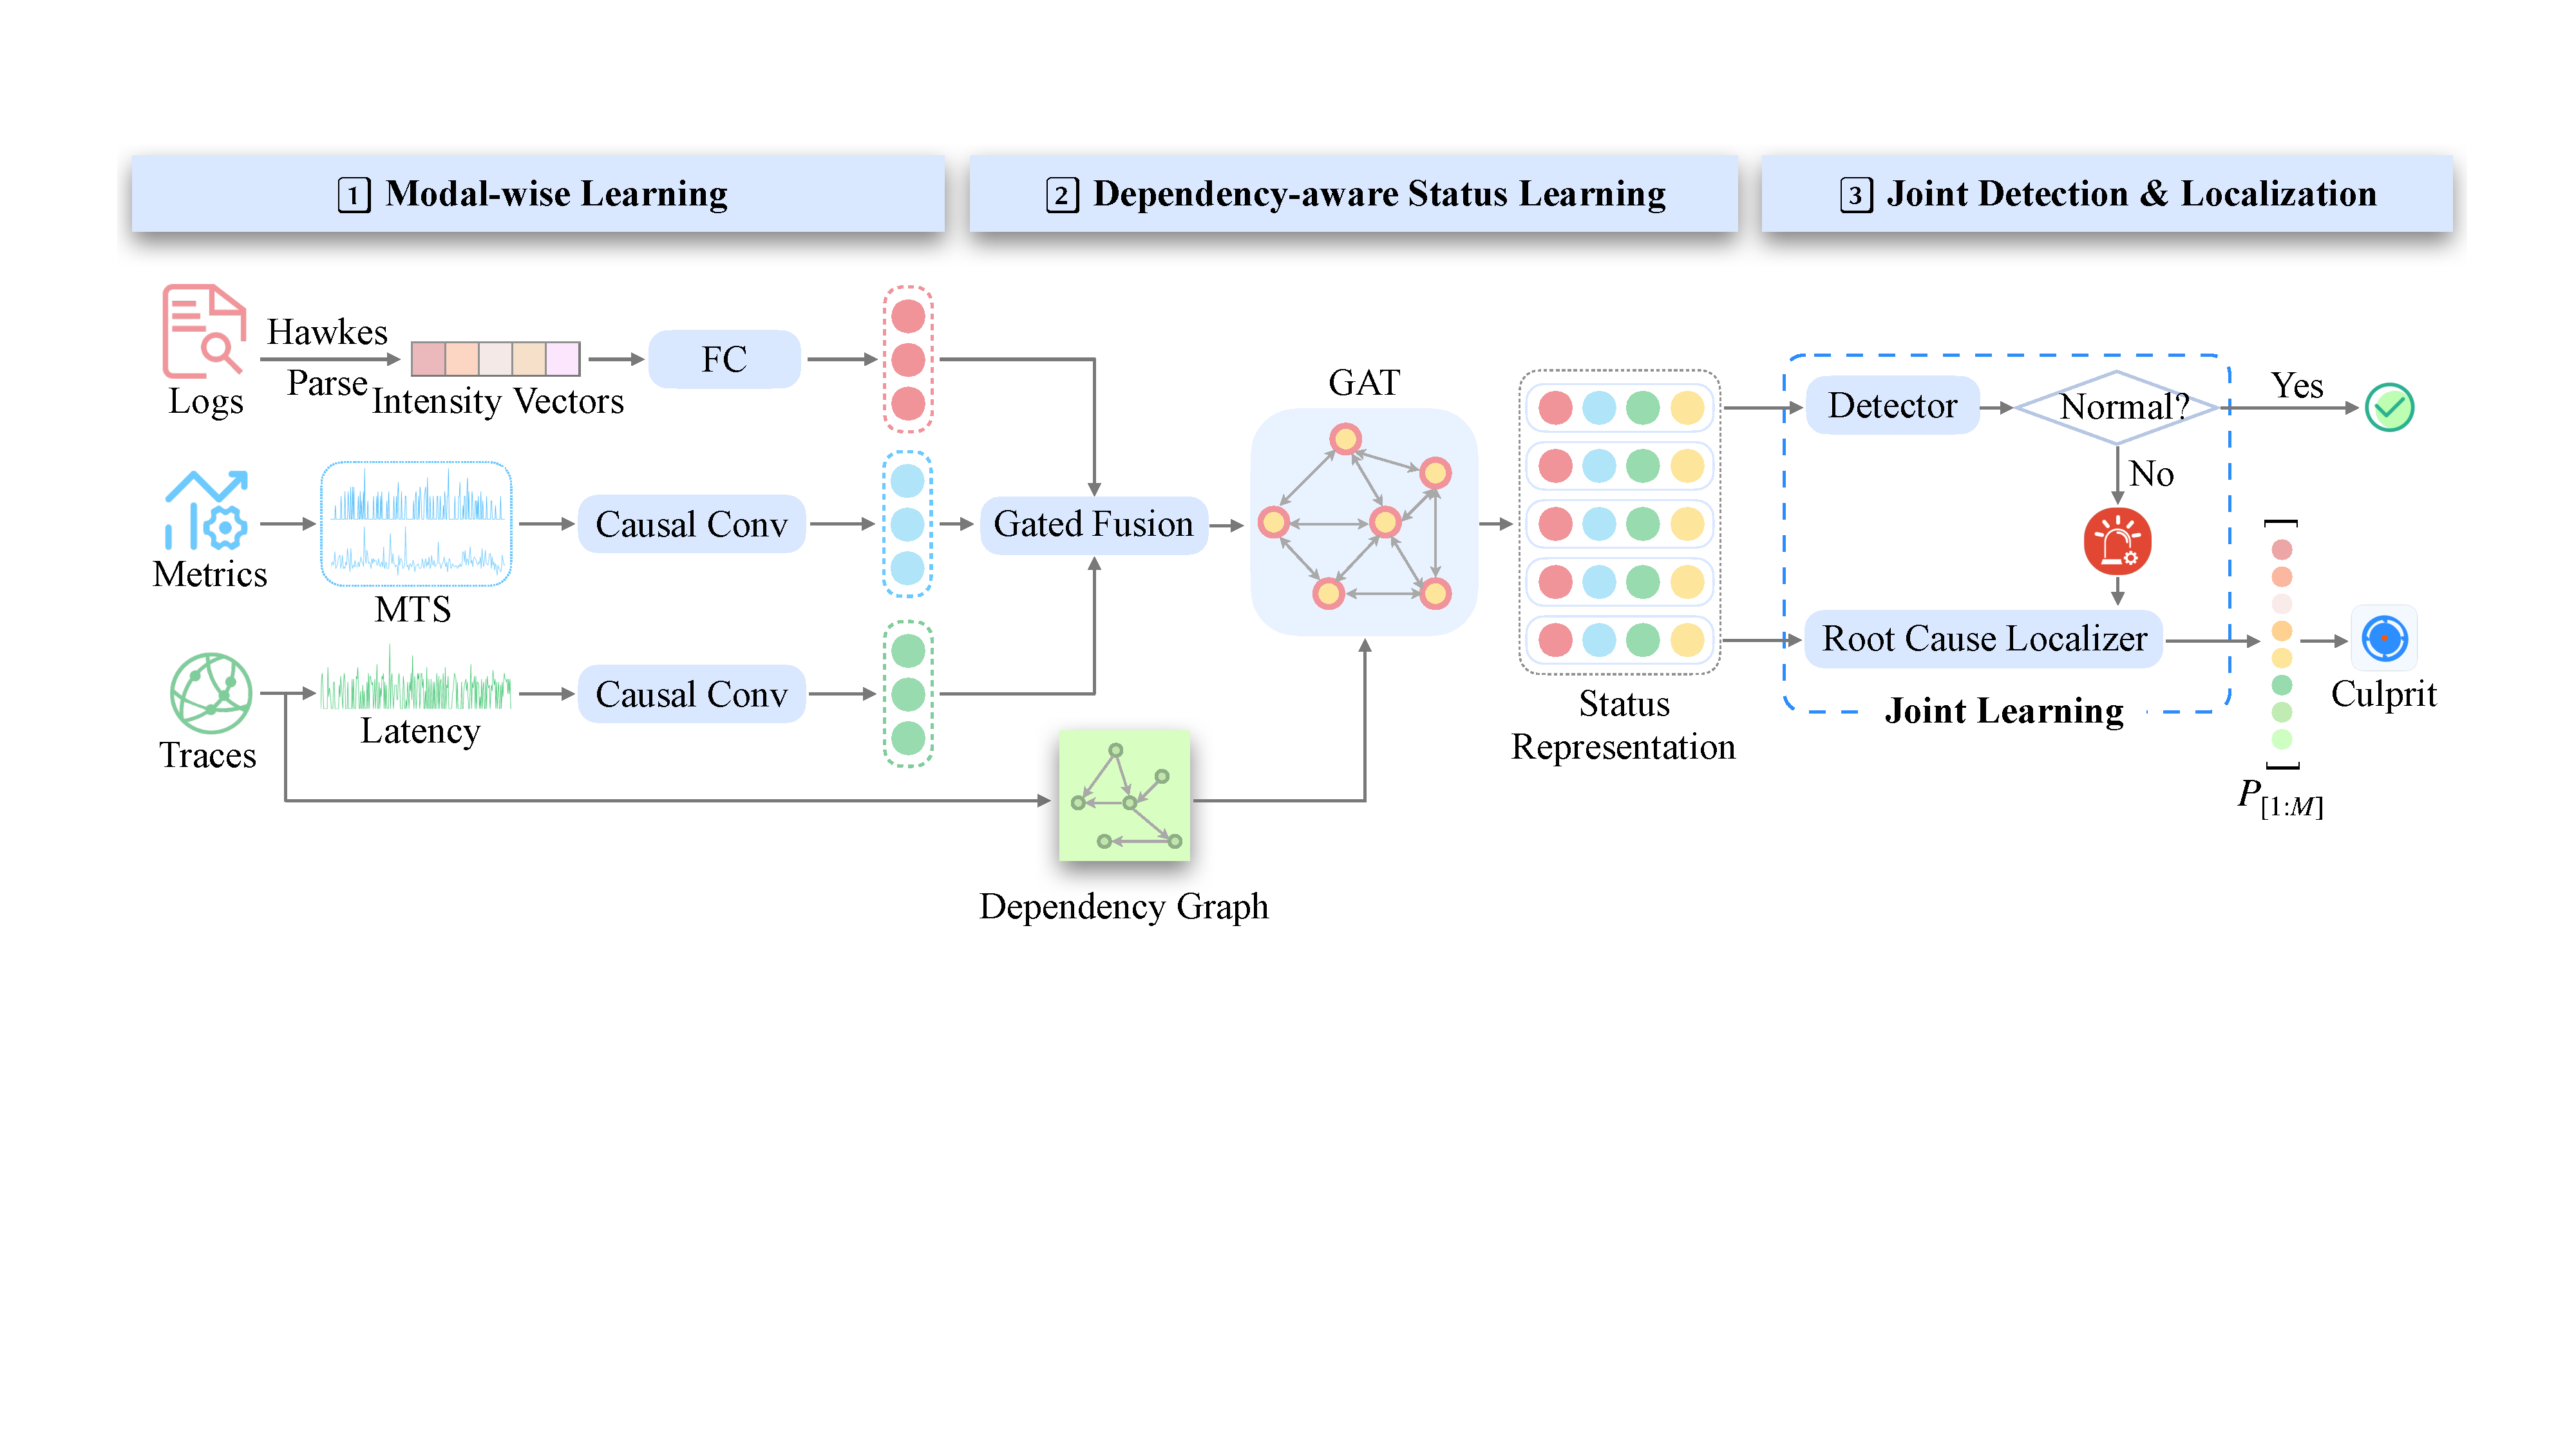
\includegraphics[width=1\linewidth]{figures/Eadro.pdf}}
    \vspace{-0.2in}
    \caption{Overview of \name}
    \label{fig:overview}
 \vspace{-0.2in}
\end{figure*}

\subsection{Modal-wise Learning}\label{sec:method:1}
This phase aims to model the different sources of monitoring data individually. We apply modality-specific models to learn an informative representation for each modality.

\subsubsection{Log Event Learning}\label{sec:method:log}
We observe that both log semantics and event occurrences can reflect anomalies (\cref{sec:study:multi-source}), yet we herein focus on event occurrences because of two reasons: 
1) the logging behavior of microservices highly relies on the developers' expertise, so the quality of log semantics cannot be guaranteed~\cite{SurveyHe};
2) the complexity of microservices necessitates lightweight techniques.
As semantic extraction requires computation-intensive natural language processing technologies, log semantic-based methods may pose challenges in practical usage.

Therefore, we focus on modeling the occurrences of log events instead of log semantics. 
An insight facilitates the model. We observe that the past event increases the likelihood of the event's occurrence in the near future, which fits the assumption of the self-exciting process~\cite{self-exciting}. 
Hence, we initially propose to adopt the Hawkes process~\cite{Hawkes}, a kind of self-exciting point process, to model the event occurrences, which is defined by the conditional intensity function:
\begin{equation}\label{eq:hawkes}
    \lambda_l^*(t) = \mu_l(t)+\sum_{\tau < t} \phi_l(t-\tau)
\end{equation}
where $l=1,...,L$ and $L$ is the number of event types; for the $l$-th event, $\mu_l$ is an estimated parameter and $\phi_l (\cdot)$ is a user-defined triggering kernel function. 
We use an exponential parametrisation of the kernels herein following~\cite{HawkesADM4}: $\phi_l (\cdot) = \alpha_l\beta \exp(-\beta t)|_{t>0}$, where $\alpha_1 \cdots \alpha_L$ are estimated parameters and $\beta$ is a hyper-parameter.

In brief, log learning is done in a three-step fashion:
\begin{itemize}[leftmargin=12pt, topsep=3pt]
\setlength\itemsep{0.4em}
\item[A.] Parsing: \name starts with parsing logs into events via Drain~\cite{Drain} by removing variables in log messages.

\item[B.] Estimating: we then record the timestamps of event occurrences (relative to the starting timestamp of the observation window) to estimate the parameters of the Hawkes model with an exponential decay kernel. The estimation is implemented via an open-source toolkit Tick~\cite{tick}.
In this way, events $\mathbf{X}^\mathcal{L}$ at each microservice inside a window are transformed into an intensity vector $\boldsymbol{\Lambda}=[\lambda_1^*,\cdots,\lambda_L^*] \in \mathbb{R}^L$. 

\item[C.] Embedding: the intensity vector $\boldsymbol{\Lambda}$ is embedded into a dense vector $\boldsymbol{H}^\mathcal{L} \in \mathbb{R}^{E^\mathcal{L}}$ in the latent space via a fully connected layer with the hidden size of ${E^\mathcal{L}}$.
\end{itemize}

\subsubsection{KPI Learning}\label{sec:method:KPI}
We first organize the KPIs $\mathbf{X}^\mathcal{K}$ with $k$ indicators of each microservice into a $k$-variate time series with the length of $T$.
Then we use a 1D dilated causal convolution (DCC)~\cite{TCN} layer that is lightweight and parallelizable to learn the temporal dependencies and cross-series relations of KPIs. 
Previous studies have demonstrated DCC's computational efficiency and accuracy in feature extraction of time series~\cite{TCNexp}.
Afterward, we apply a self-attention~\cite{Attn} operation to compute more reasonable representations, and the attention weights are as computed in Equation~\ref{eq:attn}.
\begin{equation}\label{eq:attn}
    Attn(X) = \mathsf{softmax} \left( \frac{W_qX \cdot (W_kX)^{\mathrm{T}}}{\sqrt{d}}(W_vX) \right) 
\end{equation}
where $W_q$, $W_k$, and $W_v$ are learnable parameters, and $d$ is an empirical scaling factor.
This phase outputs $\boldsymbol{H}^\mathcal{K} \in \mathbb{R}^{E^\mathcal{K}}$ representing KPIs, where $E^\mathcal{K}$ is the number of convolution filters.

\subsubsection{Trace Learning}\label{sec:method:trace}
Inspired by previous works~\cite{AID, DyCause, TraceAnomaly}, we extract latency from trace files and transform it into a time series by calculating the average latency at a time slot for each callee. We obtain a $T$-length univariate latency time series at each microservice (i.e., callee).
Similarly, the latency time series is fed into a 1D DCC layer followed by a self-attention operation to learn the latent representation $\boldsymbol{H}^\mathcal{T} \in \mathbb{R}^{E^\mathcal{T}}$, where $E^\mathcal{T}$ is the pre-defined number of filters.
Note that we simply pad time slots without corresponding invocations with zeros.

\subsection{Dependency-aware Status Learning}\label{sec:method:2}
In this phase, we aim to learn microservices' overall status and draw a comprehensive picture of the system. This module consists of three steps: dependency graph construction, multi-modal fusion, and dependency graph modeling.
We first extract a directional graph depicting the relationships among microservices from historical traces. 
Afterward, we fuse the multi-modal representations obtained from the previous phases into latent node embeddings to represent the service-level status. Messages within the constructed graph will be propagated through a graph neural network so as to learn the neighboring dependencies represented in the edge weights. 
Eventually, we can obtain a dependency-aware representation representing the overall status of the microservice system.

\subsubsection{Dependency Graph Construction}
By regarding microservices as nodes and invocations as directional edges, we can extract a dependency graph $\mathcal{G}=\{\mathbb{V}, \mathbb{E}\}$ from historical traces to depict the dependencies between microservices. 
Specifically, 
$\mathbb{V}$ is the node set and $|\mathbb{V}|=M$, where $M$ is the number of microservices; 
$\mathbb{E}$ is the set of edges, and $\vec{e}_{a,b}=(v_a, v_b) \in \mathbb{E}$ denotes an edge directed from $v_a$ to $v_b$, that is, $v_b$ has invoked $v_a$ at least once in the history.

\subsubsection{Multi-modal Fusion}\label{sec:method:fuse}
In general, there are three fusion strategies~\cite{fusion}: early fusion carried out at the input level, intermediate fusion for fusing cross-modal representations, and late fusion at the decision level (e.g., voting). 
Research in cross-modal learning ~\cite{feifei14fusion, NIPS16fusion} and neuroscience~\cite{Neuro19fusion, Multisensory21fusion} suggests that intermediate fusion usually facilitates modeling, so we transform single-modal representations to a compact multi-modal representation via intermediate fusion.

The fusion contains two steps:
\begin{itemize}[leftmargin=12pt, topsep=3pt]
\setlength\itemsep{0.4em}
\item[A.] We concatenate ($[\cdot || \cdot]$) all representations of each microservice obtained from the previous phase to retain exhaustive information. 
The resulting vector $[\boldsymbol{H}^\mathcal{L} || \boldsymbol{H}^\mathcal{K} || \boldsymbol{H}^\mathcal{T}]$ is subsequently fed into a fully connected layer to be projected into a lower-dimensional space, denoted by $\boldsymbol{H}^{\prime \mathcal{S}} \in \mathbb{R}^{2E}$, where $2E < E^\mathcal{L}+E^\mathcal{K}+E^\mathcal{T}$ is an even number.

\item[B.] $\boldsymbol{H}^{\prime \mathcal{S}}$ passes through a Gated Linear Unit (GLU)~\cite{GLU} to fuse representations in a non-linear manner and filter potential redundancy.
GLU controls the bandwidth of information flow and diminishes the vanishing gradient problem. It also possesses extraordinary resilience to catastrophic forgetting. 
As we have massive data and complex stacked neural layers, GLU fits our scenario well. 
The computation follows $\boldsymbol{H}^\mathcal{S} = GLU(\boldsymbol{H}^{\prime \mathcal{S}}) = \boldsymbol{H}^{\prime \mathcal{S}}_{(1)} \otimes \sigma(\boldsymbol{H}^{\prime \mathcal{S}}_{(2)})$, where $\boldsymbol{H}^{\prime \mathcal{S}}_{(1)}$ is the first half of $\boldsymbol{H}^{\prime \mathcal{S}}$ and $\boldsymbol{H}^{\prime \mathcal{S}}_{(2)}$ is the second half; $\otimes$ denotes element-wise product, and $\sigma$ is a sigmoid function. 
\end{itemize}
Finally, we obtain $\boldsymbol{H}^\mathcal{S} \in \mathbb{R}^{E}$, a service-level representation of each microservice.

\subsubsection{Dependency Graph Learning}\label{sec:method:graph}
As interactions between microservices can be naturally described by dependency graphs, we apply graph neural networks to perform triage inference.
Particularly, we employ Graph Attention Network (GAT)~\cite{GAT-v2} to learn the dependency-aware status of the microservice system.
GAT enables learning node and edge representations and dynamically assigns weights to neighbors without requiring computation-consuming spectral decompositions.
Hence, the model can pay attention to microservices with abnormal behaviors or at the communication hub.

The local representation $\boldsymbol{H}^\mathcal{S}$ serves as the node feature, and GAT learns the whole graph's representation, where dynamic weights of edges are computed as Equation~\ref{eq:gat}.
\begin{equation}\label{eq:gat}
    \omega_{a,b} = \frac{\exp(\mathsf{LeakyReLU}
    (v^\mathrm{T}
    [\boldsymbol{W}\boldsymbol{H}_a^\mathcal{S} || \boldsymbol{W}\boldsymbol{H}_b^\mathcal{S}]))}
    {\sum_{k \in \mathbb{N}_a} 
    \exp(\mathsf{LeakyReLU}(v^\mathrm{T}
    [\boldsymbol{W}\boldsymbol{H}_a^\mathcal{S} || \boldsymbol{W}\boldsymbol{H}_k^\mathcal{S}]))}
\end{equation}
where $\omega_{a,b}$ is the computed weight of edge $\vec{e}_{a,b}$;
$\mathbb{N}_a$ is the set of neighbor nodes of node $a$; $\boldsymbol{H}_a^\mathcal{S}$ is the inputted node feature of $a$; 
$\boldsymbol{W} \in \mathbb{R}^{E^\mathcal{G} \times E}$ and $v \in \mathbb{R}^{2E^\mathcal{G}}$ are learnable parameters.
$E^\mathcal{G}$ is the dimension of the outputted representation, which is calculated by $\boldsymbol{\hat{H}}_a^{\mathcal{S}} = \psi (\sum_{b \in \mathbb{N}_a} \omega_{a,b} \boldsymbol{W}\boldsymbol{H}_b^{\mathcal{S}})$, where $\psi(\cdot)$ is a customized activation function, usually ReLU.
Eventually, we perform global attention pooling~\cite{GAP} on the multi-modal representations of all nodes. The final output is $\boldsymbol{H}^\mathcal{F} \in \mathbb{R}^{E^\mathcal{F}}$, a dependency-aware representation of the overall system status.

\subsection{Joint Detection and Localization}\label{sec:method:output}
Lastly, \name predicts whether the current observation window is abnormal and if so, it identifies which microservice the root cause is.
As demonstrated in~\cref{sec:study:detection}, existing troubleshooting methods regard anomaly detection and root cause localization as independent and ignore their shared knowledge. 
Besides, current anomaly detectors deliver unsatisfactory results and affect the next-stage localization by incorporating noisy labels.
Therefore, we fully leverage the shared knowledge and integrate two closely related tasks into an end-to-end model.
\begin{figure}[htb]
    \centering
    \vspace{-0.1in}
        {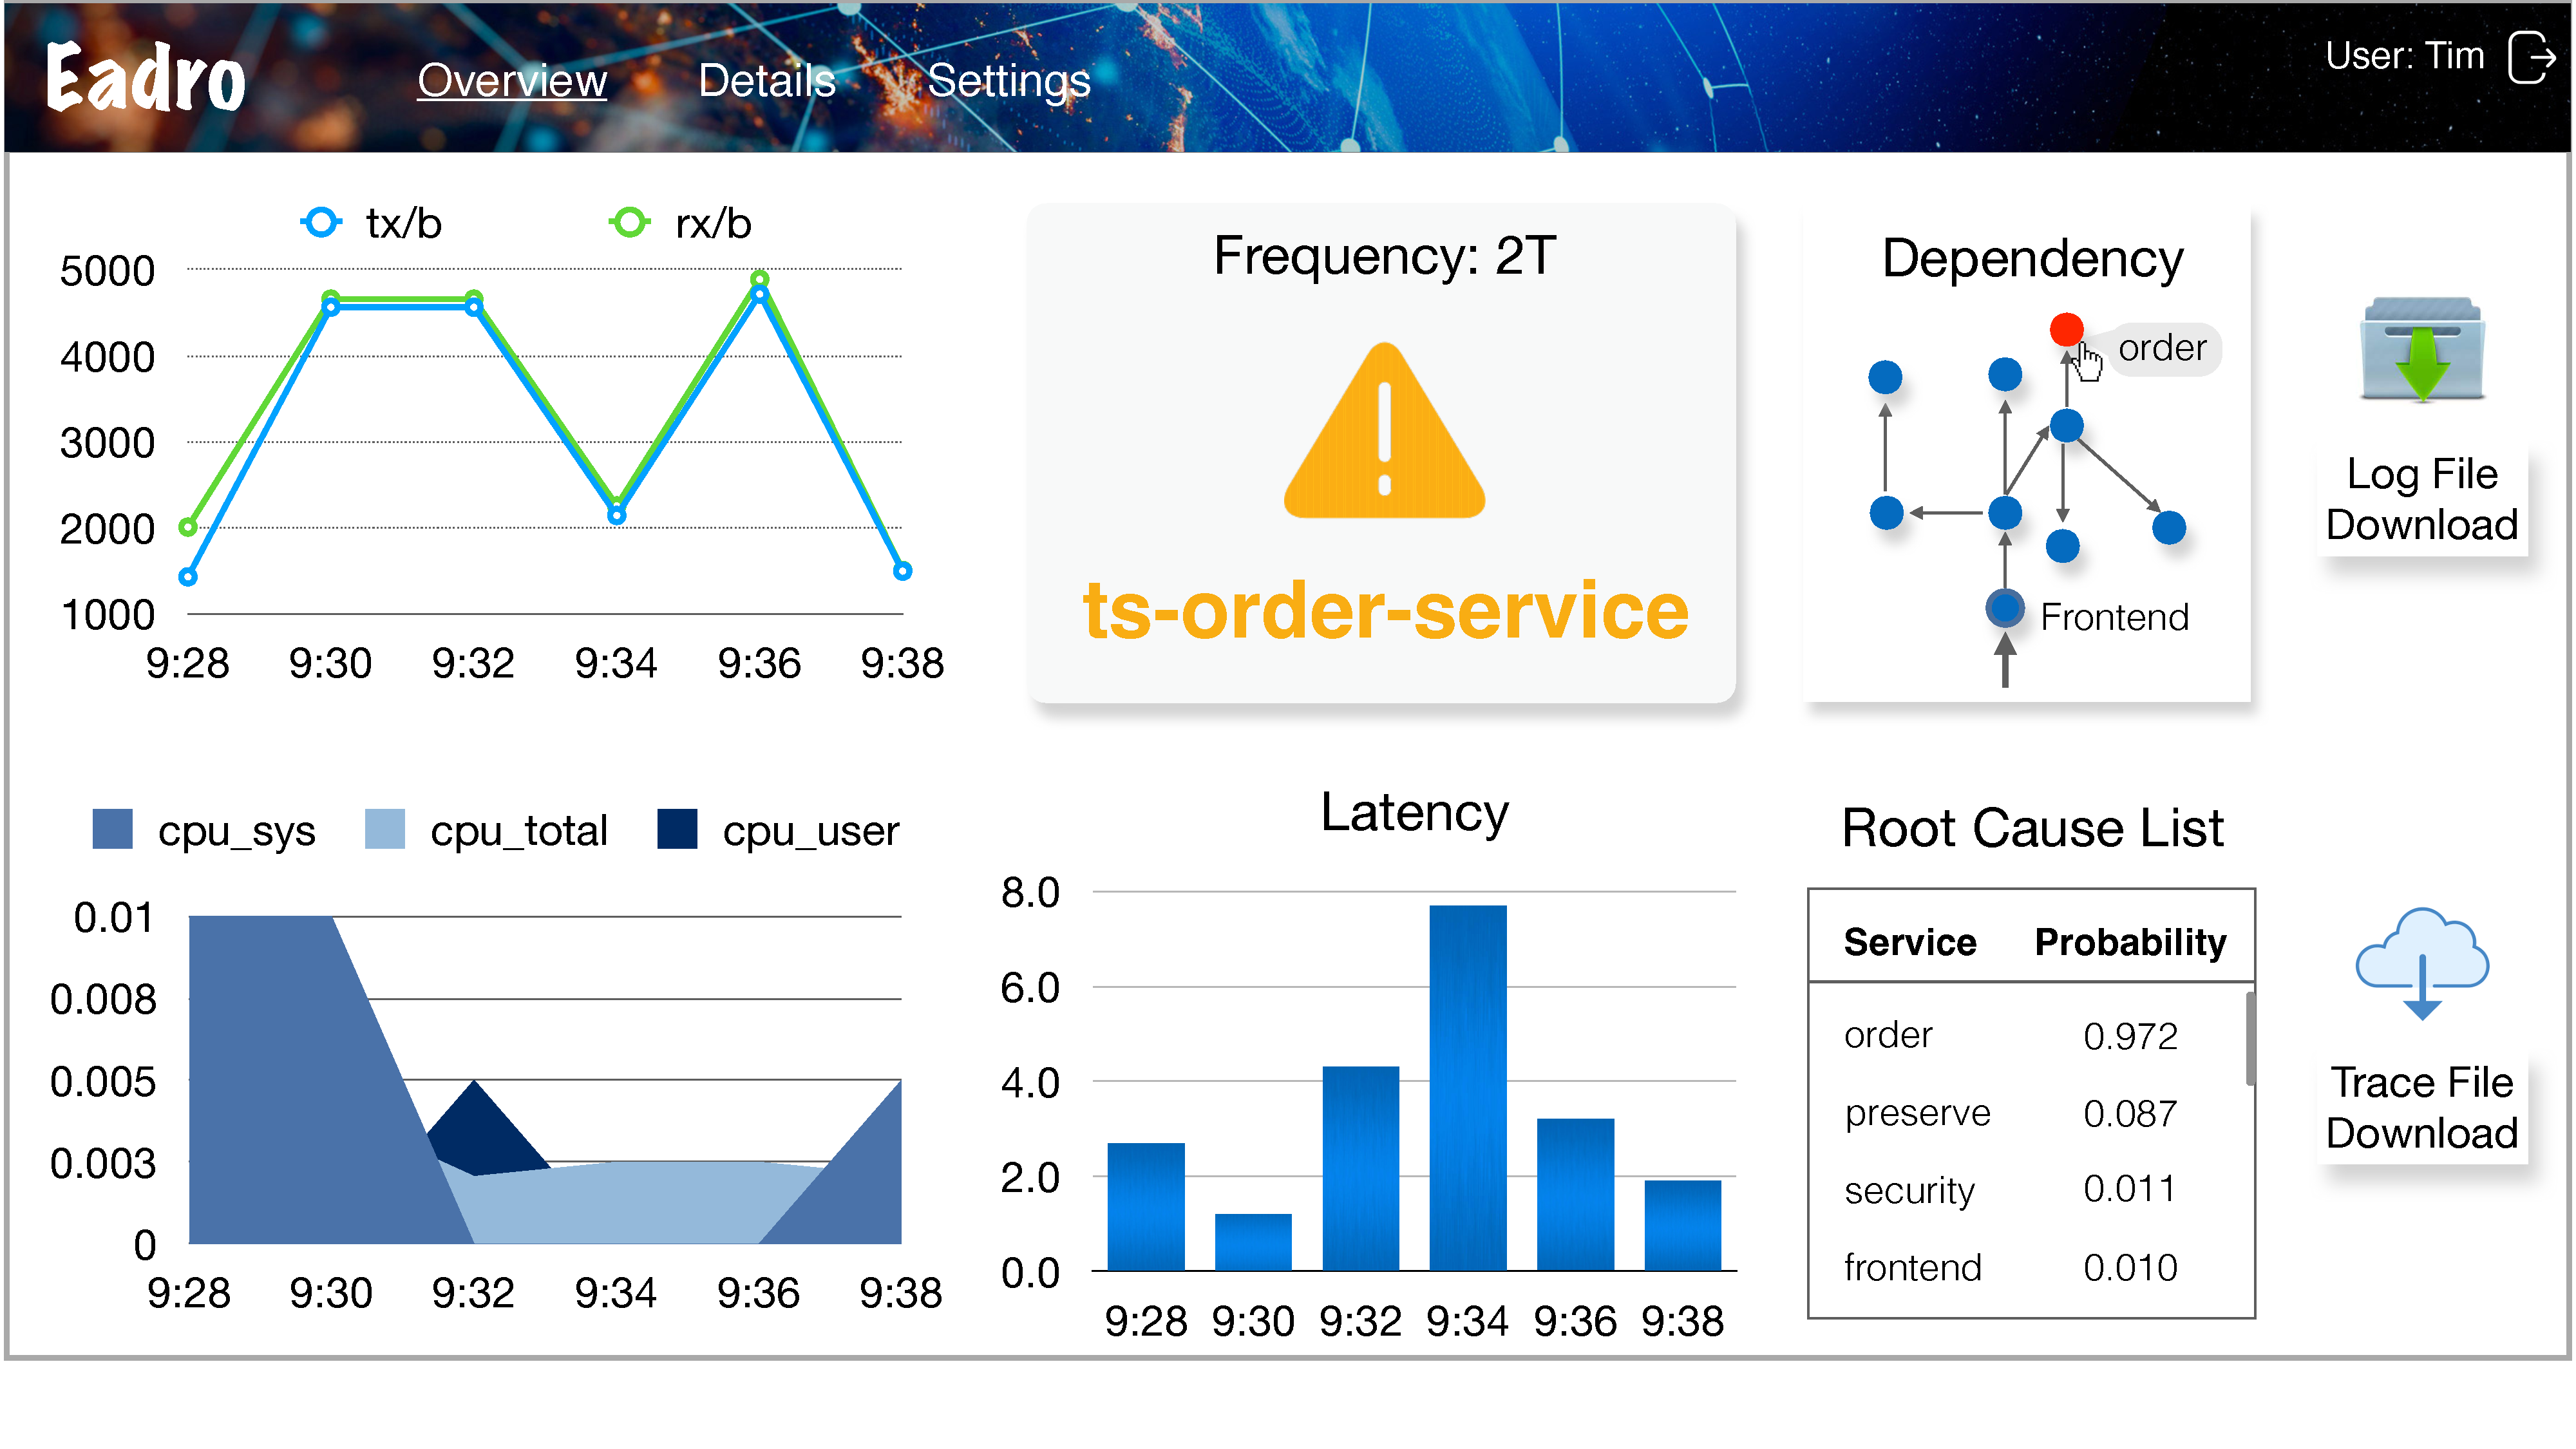
\includegraphics[width=0.99\linewidth]{figures/interface.pdf}}
    \vspace{-0.2in}
    \caption{A demo for reviewing the suspicious status.}
    \label{fig:interface}
\vspace{-0.1in}
\end{figure}

In particular, based on the previously obtained representation $\boldsymbol{H}^\mathcal{F}$, a detector first conducts binary classification to decide the existence of anomalies.
If no anomaly exists, \name directly outputs the result; if not, a localizer ranks the microservices according to their probabilities of being the culprit.
The detector and the localizer are both composed of stacked fully-connected layers and jointly trained by sharing an objective.
The detector aims to minimize the binary cross-entropy loss:
\begin{equation}\label{eq:loss-detection}
    \mathfrak{L}_1 = \sum_{i=1}^N [-(y_i\log(\hat{y_i}) + (1-y_i)\log(1-\hat{y_i}))]
\end{equation}
where $N$ is the number of historical samples; $y_i \in \{0,1\}$ is the ground truth indicating the presence of anomalies (1 denotes presence while 0 denotes absence), and $\hat{y_i} \in [0,1]$ is the predicted indicator.
Subsequently, all samples predicted as normal (0) are masked, and samples predicted as abnormal (1) pass through the localizer. 
The localizer attempts to narrow the distance between the predicted and ground-truth probabilities, whose objective is expressed by:
\begin{equation}\label{eq:loss-localization}
    \mathfrak{L}_2 = \sum_{i=1}^N \sum_{s=1}^M c_{i, s} \log (p_{i,s})
\end{equation}
where $M$ is the number of involved microservices. In the $i$-th sample, $c_{i,s} \in \{0,1\}$ is 1 if the culprit microservice is $s$ and 0 otherwise; $p_{i,s}$ is the predicted probability of microservice $s$ being the culprit.
The objective of \name is the weighted sum of the two sub-objectives $\mathfrak{L} = \beta \cdot \mathfrak{L}_1 + (1-\beta) \cdot \mathfrak{L}_2$, where $\beta$ is a hyper-parameter balancing the two tasks.
Eventually, \name outputs a ranked list of microservices to be checked according to their predicted probabilities of being the root cause.

To sum up, \name can provide explicit clues about the microservice status. Hence, troubleshooting is much more convenient for operation engineers with the ranked list of microservices.
Figure~\ref{fig:interface} presents a visualized demo.

